\section{Human Memory Model}
\label{sec:memory_model}

Dual-process theory of memory proposes that the brain stores both \emph{verbatim} and \emph{gist} representations of an event.  Since we will be focusing on intelligence factoids that contain specific details about a situation, which may also be obtained from another person and not from directly witnessing an event firsthand, we will exclusively consider the recall of verbatim traces.  

While a large number of factors can impact the encoding, storage, and recall of memories, we choose in this work to focus on only three well-studied components:  working memory capacity, the serial position effect, and bias encoding.  We address each of these factors' effects on the ability of recalling intelligence factoids.

\subsection{Working Memory Capacity}

The capacity of a persons' working memory is dependent on a few factors, such as the specific individual and the type of information being stored.  The variance in these differences of various memory capacities, however, is relatively small.  We can define the capacity of individual $x$ in a specific scenario as $K_x$ elements, where $K_x$ is a normal random variable given by $K_x = N( \mu_K, \sigma_K )$, where $\mu_k = U(\mu_{K_{min}},\mu_{K_{max}})$ is given by a uniform random variable with a defined minimum and maximum value and $\sigma_K$ is a given constant taken from empirical evaluations.  Using this model, different individuals' average capacities can be captured as well as the randomness of the capacity at various times or situations.

Since $K_x$ represents the likelihood of recalling each factoid, $i$ will partially depend on how many total factoids are presented.  Specifically, 

Question: Should the expected number of recall items should equal the capacity?:
\begin{equation}
	E [ \sum\limits_{i=1}^N R_{i}^x ] = K_x
\end{equation}
%If so, should that hold for all $N$?  For example, if my working memory capacity is $\approx 10$, do I remember $10$ things on average when 

\subsection{Serial Position Effect}
\label{sec:ser_pos_effect}

\begin{figure}
\begin{centering}
    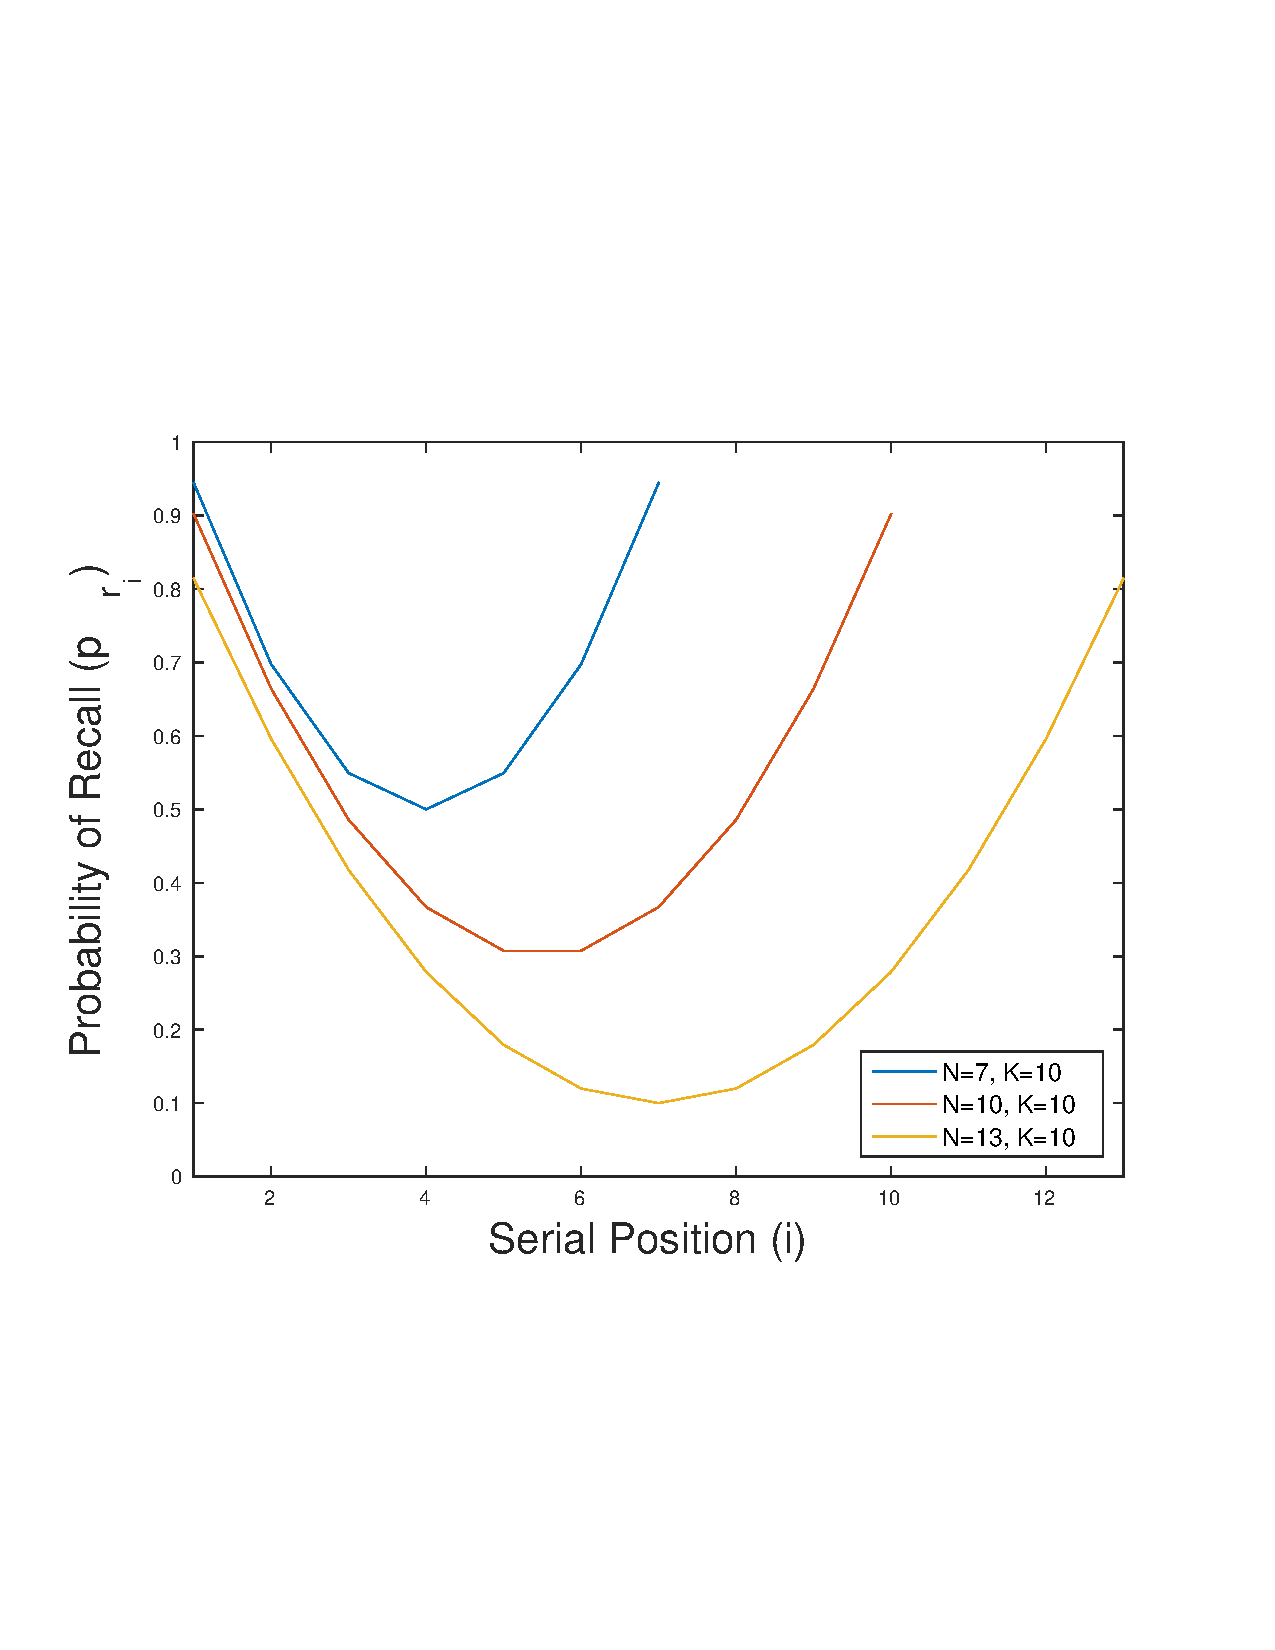
\includegraphics[clip=true, trim = 0mm 65mm 25mm 50mm, scale=0.50]{figures/mean_prob_recall_vs_ser_pos.pdf}
    \caption{ The mean probability of recall is impacted by the serial position effect and the amount of information relative to capacity. }
    \label{fig:prob_recall_vs_serial_pos}
\end{centering}
\end{figure}

The serial position effect describes the phenomenon by which people are more likely to recall the information presented to them first and last in a sequence than the information in the middle of the sequence.  Given $N$ and $K$, we can define a function for $p_{r_i} = f(N,K,i)$.  Figure \ref{fig:prob_recall_vs_serial_pos} shows examples of this function for an instance of $K=10$ and several example values of $N$ illuminating each possibility of $N < K$, $N = K$, and $N > K$.

Question:  The function used to generate the examples of $p_{r_i}$ is just a scaled parabola of the form:
\begin{equation}
    	f(N,K,i) = \frac{(i - \frac{N+1}{2})^2}{(\frac{N+1}{2} + p_{r_i-min})^2} + p_{r_i-min}
\end{equation}
where $\frac{N+1}{2}$ centers the function relative to $N$ and $p_{r_i-min}$ is a chosen value representing the minimum probability of recalling any item.
Are there any references that provide actual functions of the serial position effect data that we should use?  If not, meaning we do need to use a function that models it as best as we can, how close is this?  Should it be weighted more heavily on one side or the other, for example?

\subsection{Bias Encoding}

Question:  How can we incorporate this into the model?  

Proposal:  We can define subject areas $\mathcal{S} = \{S_1, ...S_M\}$.  An agent can be an expert (or familiar) with some subset of these subject areas, and each factoid can also be defined to belong to a subset of the subject areas.  Then we could introduce a scaling factor based on the overlap between an agent's area of expertise and how the factoid fits into it.  Is there any basis for this kind of thing in memory research?

\subsection{Note on $p_{r_i}$}
Here, I am defining $p_{r_i}$ to be a constant probability based on the values of $N$, $K$, and $i$.  An alternative that might make it more realistic, but possibly complicate analysis, would be to have it be a random variable itself.  It could be given by $N(\mu_{r_i}, \sigma_{r_i})$ where $\mu_{r_i}$ is given by a function of $N$, $K$, and $i$, just as $p_{r_i}$ is treated above.  

